\subsection{Word Segmentation}
\label{sec:cws}

\subsubsection{CRF}
\label{sec:crf}

条件随机场~\cite{lafferty2001conditional}是一种无向概率图模型,常用在序列标注问题中。

条件随机场是在给定的随机变量 X (观测序列 $o_{1}, \cdots, o_{i}$) 条件下,随机变量 Y (隐状态序列 $i_{1}, \cdots, i_{i}$ 的马尔科夫随机场。

条件随机场是一种无向概率图模型,在迭代过程中,通过寻找最大团块(子图中任意两点间都有边相邻)进行参数消除。
无向图的联合概率值等于所有最大团块的势函数乘积除以归一化因子。
这就意味着条件随机场是一个全局迭代的过程,其结果要等到最后才能知道,所造成的迭代效率也就偏低。

在实验过程中, 除了使用条件随机场加上一些词嵌入方法之外,还用了分词任务中常见的BiLSTM加上条件随机场CRF进行处理。

我们将序列标注问题转化为概率图模型,这就导致了概率图的输入值对结果起到了至关重要的影响。

条件随机场的条件概率和归一化因子如下:

$P(I|O) = \frac{1}{Z(O)}exp( \sum_{i,k}^{}{\lambda_{k}}t_{k}(O_{i-1},O_{i},I,i)+\sum_{i,l}^{}{\mu_{l}}I_{l}(O_{i},I,i) )$

$Z(O)= \sum_{I}^{}{exp( \sum_{i,k}^{}{\lambda_{k}}t_{k}(O_{i-1},O_{i},I,i)+\sum_{i,l}^{}{\mu_{l}}I_{l}(O_{i},I,i) )}$

条件概率$P(y|x)$表示了在给定的一条观测序列 $O=(o_{1},\cdots, o_{i})$ 条件下,CRF求出隐状态序列 $I=(i_{1},\cdots, i_{i})$ 的概率值。

展开上式,得到:

$P(I | O)=\frac{1}{Z(O)} e^{\sum_{i}^{T}\sum_{k}^{M}\lambda_{k}f_{k}(O,I_{i-1},I_{i},i)}=\frac{1}{Z(O)} e^{ [ \sum_{i}^{T}\sum_{j}^{J}\lambda_{j}t_{j}(O,I_{i-1},I_{i},i) + \sum_{i}^{T}\sum_{l}^{L}\mu_{l}s_{l}(O,I_{i},i) ] }$


其中:

$t_{j}$ 为第i状态的转移到j状态特征,对应权重 $\lambda_{j}$

$s_i$为第i个的状态特征,对应权重$μ_i$, 其用来表示是否满足label条件,用来打分评价该隐状态的权值。

然后对Score进行求和归一化得到其概率值。

\subsubsection{BiLSTM CRF}
\label{sec:bilstm_crf}

如果我们用单模型,既在给定特征的基础上做一个最大概率分布计算,那么我们相当于假定我们的特征能很好的表示当前上下文信息,能表示需要分词的Context。

但实际上并不是这样的,首先One-Hot可以直观的感觉,它只是学习到某些特定的词组合,并没有学习到词义层级的信息。

即使是用Tf-idf,甚至采用预训练的词嵌入作为输入,也不能较好的表示上下文信息,容易丢失一些局部的特征,学习到的效果较为死板。
而使用预训练获得的词向量表示容易放大原本的噪声,因为条件随机场是一种全局化最优隐层状态概率值,原有的噪音会被放大导致不太好的效果。
所以一般单条件随机场模型在分词问题上效果一般。

通过双向LSTM获得上下文信息,从而使得概率图CRF的输入噪音较小。继而获得更好的学习效果,

而对比单纯使用BiLSTM的模型,CRF层在BiLSTM表示Context信息的基础上做了一个选择最大概率分类的工作。
通过无向概率图模型的,选择概率最大的最优label路径,可以明提升模型效果。


\begin{figure*}[htbp!]
    \begin{center}
    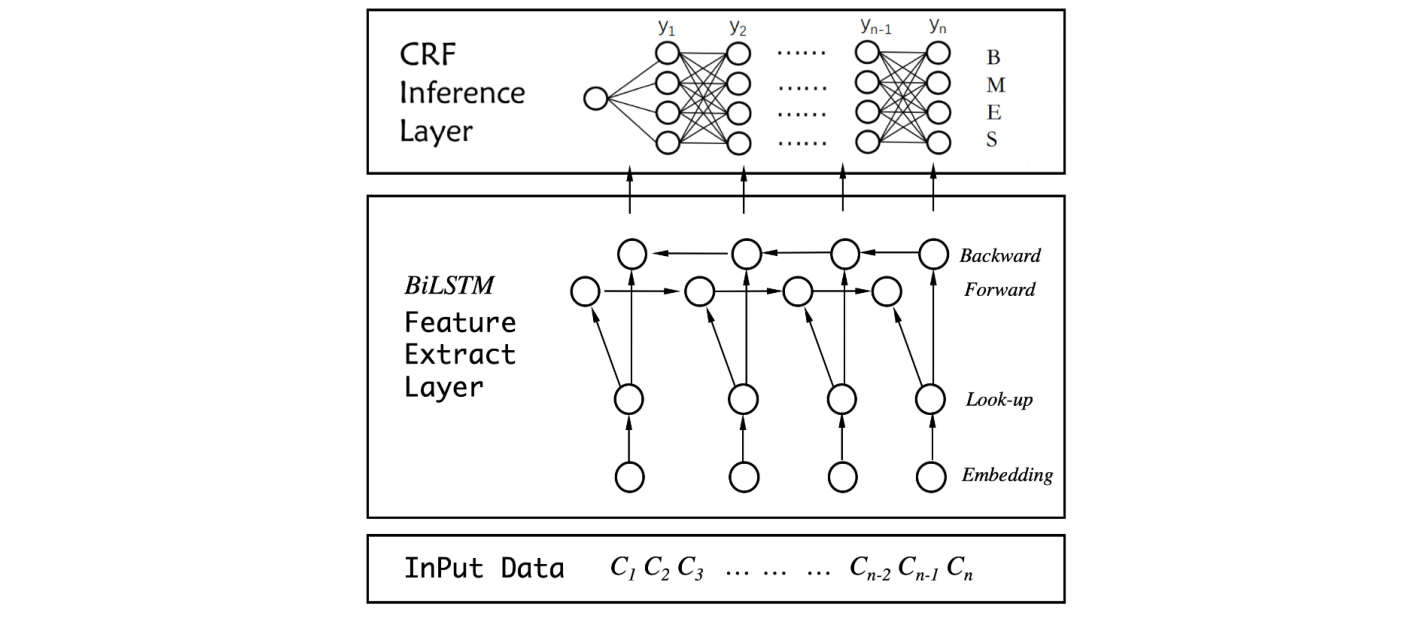
\includegraphics[width=1\textwidth]{figures/model.pdf}
    \end{center}
    \caption{The overview of BiLSTM-CRF model structure}
    \label{fig:overall_model}
\end{figure*}